%
% File acl2020.tex
%
%% Based on the style files for ACL 2020, which were
%% Based on the style files for ACL 2018, NAACL 2018/19, which were
%% Based on the style files for ACL-2015, with some improvements
%%  taken from the NAACL-2016 style
%% Based on the style files for ACL-2014, which were, in turn,
%% based on ACL-2013, ACL-2012, ACL-2011, ACL-2010, ACL-IJCNLP-2009,
%% EACL-2009, IJCNLP-2008...
%% Based on the style files for EACL 2006 by 
%%e.agirre@ehu.es or Sergi.Balari@uab.es
%% and that of ACL 08 by Joakim Nivre and Noah Smith

\documentclass[11pt,a4paper]{article}
\usepackage[hyperref]{acl2020}
\usepackage{times}
\usepackage{todonotes}
\usepackage{latexsym}
\renewcommand{\UrlFont}{\ttfamily\small}

% This is not strictly necessary, and may be commented out,
% but it will improve the layout of the manuscript,
% and will typically save some space.
\usepackage{microtype}

\aclfinalcopy % Uncomment this line for the final submission
%\def\aclpaperid{***} %  Enter the acl Paper ID here

%\setlength\titlebox{5cm}
% You can expand the titlebox if you need extra space
% to show all the authors. Please do not make the titlebox
% smaller than 5cm (the original size); we will check this
% in the camera-ready version and ask you to change it back.

\newcommand\BibTeX{B\textsc{ib}\TeX}

\title{Covid Quarantino: A GPT-based Conversational Chatbot}

\author{Felipe Moreno \\
  \texttt{pipemon@mit.edu} \\\And
  Juan Ferrua \\
  \texttt{juangelo@mit.edu} \\}

\date{}

\begin{document}
\maketitle
\begin{abstract}

NLP models designed for question answering or conversational capabilities are usually centered on task-specific applications and designed to focus on the most recent question input. Our vision is that several task-specific models can be combined with a general conversational model to provide a better experience for its users. We demonstrate with Covid Quarantino that this type of system can lead to a valuable combination of answering subject-specific questions and providing general conversational capabilities. To create Covid Quarantino, we combined a generative pre-trained transformer model with a framework that classifies intents and transitions control among 5 skills. We found that our model, generally, has very high recall and low accuracy.  We hope that our contribution, demonstrating the usefulness of a simple implementation, inspires future work in creating improved versions of chatbots that can better replicate written conversations with humans.

\end{abstract}


\section{Introduction}

Our inspiration stems from the lack of human interaction during the quarantine. Current chatbots excel at specific task-based applications, such as making restaurant reservations or answering questions about a product on a shopping site. However, they are not focused on providing a sense of continuity over different interactions, especially not if these interactions span different specific tasks. For that reason, we developed Covid Quarantino, an extensible chatbot for quarantine companionship. Our main goal was to develop a chatbot with some useful functionalities which could also provide some leisure time and entertainment. We envisioned that, in order for our chatbot to be a meaningful companion, it had to remember chat history and factor that into its responses.

\section{Our Prediction Problem, Model, and Dataset}

\paragraph{Prediction Problem}

The prediction problem we aim to fulfill is: given a string from a human user, which may be several sentences long and may or may not contain a question, as well as a history of conversational exchanges with the same user, predict a response that a human engaging in that conversation might give. Our predictions are evaluated against human-generated responses from our test dataset. Tom evaluate our chitchat model performance, used the same evaluation metrics in DialogueGPT. For the framework, we generated a test dataset of utterances which covers each possible conversation tree path twice. All of the user utterances which we used for evaluation, were not present in the training set. For evaluation, we evaluated the conversations end-to-end trying to match the conversation paths on their entirety.

\paragraph{Model}

We used Microsoft's large-scale pre-trained response generation model (DialoGPT) as the main source of Covid Quarantino's generated responses \cite{zhang2019dialogpt}. DialoGPT is an extension of OpenAI's Generative Pretrained Transformer, called GPT-2 \cite{radford2019language}. We used the large model version of DialoGPT, which has a total of 762M trainable paramaters. %\todo[inline]{mention more detail about layers and other internals}


\paragraph{Dataset} The DialoGPT model DialoGPT is trained on multi-turn conversations from Reddit discussion threads, with a total of 147M such conversations. These discussion threads span a huge range of categories, since Reddit has a community for every interest shared by a group of users. Moreover, the nature of the discussion structure often yields many replies to a given comment or question, which provides a rich set of data. \\
To fine-tune our model for our conversational use case, we used DailyDialog, a high-quality multi-turn dialog dataset \cite{li2017dailydialog}. We chose DailyDialog because the conversations are human-written and less noisy, and the dialogues are reflective of daily communication and cover various topics from our daily lives. This dataset is also manually labeled with communication intention and emotion information. We did not make use of these annotations, but they provide a natural avenue for expanding upon our current functionality. In total, it contains just over 13,000 dialogues, with an average of 7.9 speaker turns per dialogue, i.e. four back-and-forth exchanges, and an average of 114.7 tokens per dialogue. 

\section{Implementation}

\paragraph{Framework} For our chatbot framework, we used RASA, an open source machine learning framework for natural language understanding and dialogue. Rasa provides a processing pipeline for word-to-vector, text featurization, tokenization, intent classification and entity extraction and a variety of models to train to do all of the above. Rasa allows to capture intents from user text input and direct actions to a story. A story, or skill, is what we refer to as a particular functionality which allows the bot to interact with the user in a predetermined way and which could execute arbitrary code in the process like, for example, call an API, query a database or read a file. In particular, the framework allows for an out\_of\_scope intent whenever a user request does not match any of the pre-defined intents with a high confidence value. To handle those cases, we gave the chatbot the ability to engage in chitchat by generating its own responses using a dialogue generator model.

\paragraph{Pipeline}

For the pipeline, we chose to use Spacy, an open-source library for Natural Language Processing in Python, to do the tokenization, featurization and entity extraction. We use Spacy since it provides pre-trained models and requires little data for fine-tunning to our purposes. In particular, we like Spacy because it provides pre-trained given name extractors which allows our chatbot to extract the user's name and address the user by their name. 

\paragraph{Intent classifier}

For the intent classification, we used an sklearn. Sklearn's intent classifier is trained using a linear SVM which gets optimized using a grid search. We acknowledge that SVMs are not robust classifiers, but we like it because it allows us to create a classifier with just a small set of examples. The classifier also provides a detection probability for each of the pre-defined intents. 

\paragraph{Entity Extractor} We use Dual Intent and Entity Transformer (DIET) for entity extraction. 
DIET is a multi-task transformer architecture that handles both intent classification and entity recognition together. This is used in conjunction with the Sklearn's intent classifier to provide more robust intent classification. It also provides the entity extraction for our custom entities. DIET is particularly good for out application because it uses Conditional Random Fields (CRF) to calculate the Entity loss. This means that DIET is not as data hungry as other deep learning methods. DIET achieves state-of-the-art results and is a very fast training model.

\section{Skills}

We refer to the extended capabilities of our chatbot agent as skills.

\paragraph{Greet}
The greet skill uses a user greeting, such as 'Hi' or `hello' to start the skill. The chatbot agent, the first time that the skill is triggered, introduces itself to the user, mentions that it can provide a list of its functionality with a `help' command, and then proceeds to ask for the user's name. The chatbot parses out the slot corresponding to the user's name. After that point, the chatbot remembers and addresses the user by name. Future time that the greet skill is triggered, the bot won't introduce itself and will address the user by their name. Following the interaction, the greet skill will ask the user about their day in a variety of ways. The user response will be classified in either a positive or negative intent for which the chatbot responds with a corresponding empathetic gesture. In the case of a negative response, the chatbot also proposes the user to cheer their day up with a joke.

\paragraph{Comedy}
This is skill is triggered if a `comedy\_time` intent is parsed out of the user's request. It is triggered by a request such as `Tell me joke'. Then the chatbot responds to the user with a joke. We are using a dataset of Reddit jokes in English which was gathered as academic work by \cite{pungas}. All credits for this dataset goes to Pungas et al.

\paragraph{Feedback}
This is a simple single intent based skill. It is implemented to enrich the interaction with the user and to acknowledge pitfalls in the chatbot. If the user praises the chatbot, the chatbot responds thankfully. If the user scorns at the chatbot, the chatbot responds apologetically. 

\paragraph{Covid Screening}
The Covid-19 screening is a questionnaire of basic questions provided by Reid Health hospital in their website. https://www.reidhealth.org/covid-19-screening-questions
The skill is implemented as a form, a set of slots that need to be filled by the user. A `covid\_screening' intent is triggered by a user utterance such as `Covid-19 screening' or `Covid testing'. The form is activated and the chatbot starts asking the questions to the user. Each of the questions asked is a yes/no question, and each question is fulfilled with an `affirmative' or `deny' intent which maps the slot associated to the answer to a True/False boolean. After all the questions have been fulfilled, the form is `submitted' and an appropriate answer is given to the user corresponding to the given inputs. Also, independent of the responses, the chatbot mentions to the user that they should contact medical facilities ahead of time before showing up, so that medical institutions are aware of the reason of visit.

\paragraph{Chitchat}
The chitchat skill is implemented as an action to an out\_of\_scope intent. Whenever a user input's utterance is classified as intent with an accuracy (probability) less than 0.4, the utterance is regarded as an out-of-scope. Whenever this happens, the utterance is passed to the GPT model for chitchat dialogue generation. The GPT model keeps track of all of the previous chitchat requests to the model, and hence is able to maintain a dialogue conversation history for chitchatting with the user. \\
To generate a response for the user, we first encode the user input with our GPT tokenizer. We then concatenate the new tokens with the tokens from the chat history, and we pass it as an input to our GPT's encoder and decoder in order to generate the response.

\section{Experimental Results and Analysis}
We took two approaches to evaluate the performance of CovidQuarantino. First, we evaluated the classification accuracy to provide an objective measure of how well each skill performed. Second, we tested general functionality by chatting with the bot and getting a feel for the quality of its responses. 

\paragraph{Intent-entity classification accuracy} On a per-skill level, each skill written for our framework may be individually evaluated for its task. We computed the precision, recall, and f1-scores of several types of conversation interactions. These metrics are displayed in Figure 1 on the right.
\paragraph{Functionality} We had numerous conversations with Covid Quarantino to determine how well it performed relative to our anecdotal experiences texting an average stranger or acquaintance. We found that its responses were generally acceptable, but Covid Quarantino came across as a quite boring person, which was dissapointing. The engagement felt fairly low, in the sense that the responses did not give social cues of wanting to get to know us better or dive into detail about our discussion topics. Refer to Appendix A for a sample conversation with Covid Quarantino.

\begin{figure}
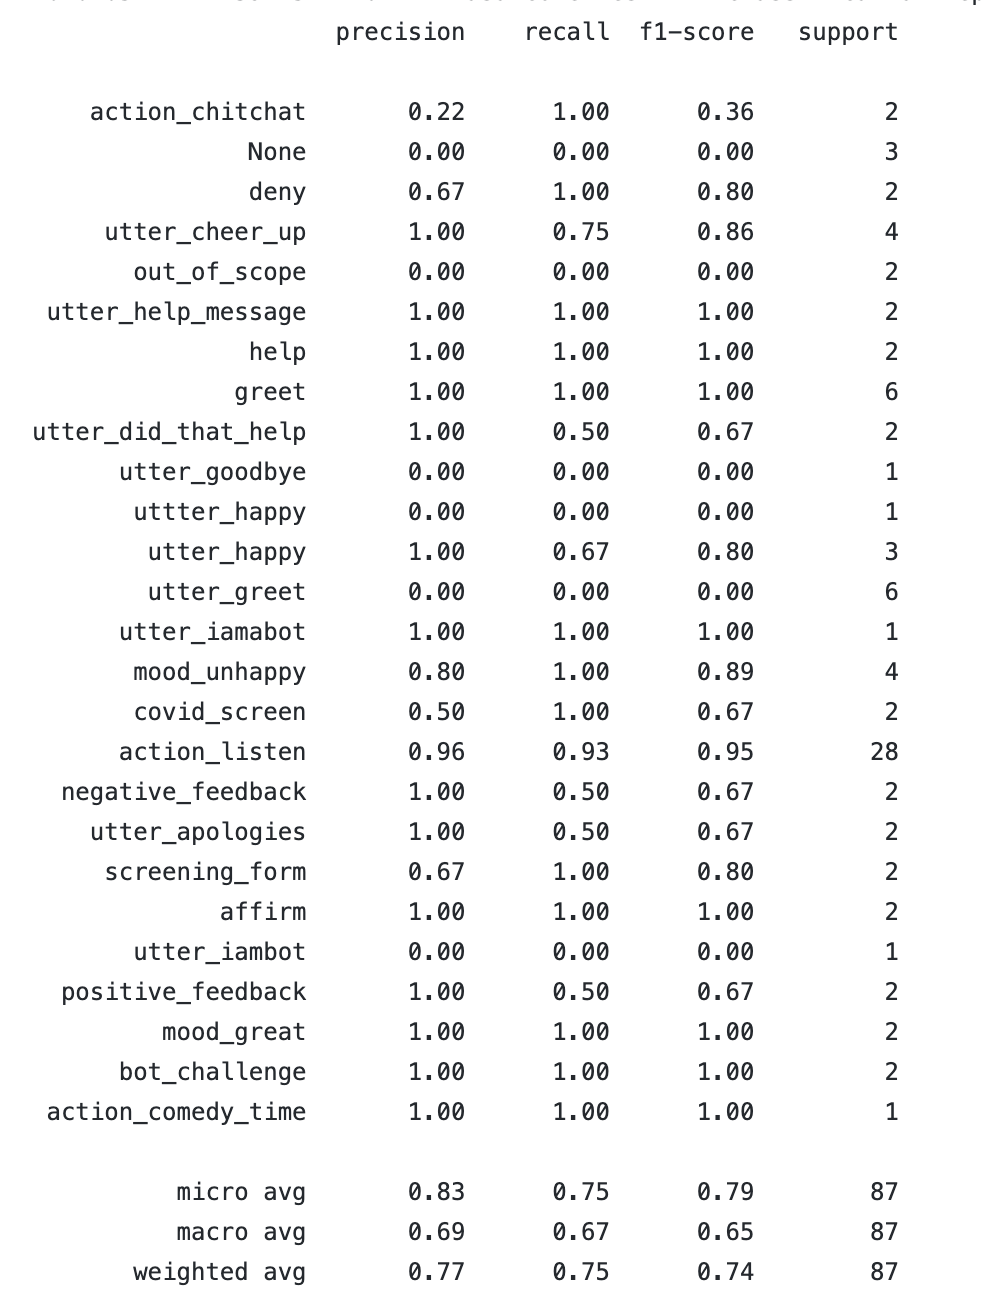
\includegraphics[scale=0.5]{evaluation_metrics.png}
\caption{Performance metrics for Covid Quarantino. The leftmost column displays the category of interactions, some of which are skills, such as \texttt{covid\_screen} and \texttt{action\_comedy\_time}, and others of which describe the general sentiment of the response called for, such as \texttt{mood\_unhappy} and \texttt{utter\_apologies}.}
\end{figure}


\section{Conclusion}

There are several avenues for future work that could improve upon the performance and capabilities of Covid Quarantino. The most obvious one is the addition of new skills to allow for new specific functionalities, which can be done easily with our framework. Second, we can improve the fine-tuning of the DialoGPT model by incorporating the intent and emotions annotations from the DailyDialog dataset. This would allow for more accurate sentiment analysis and an increased performance in generating chitchat responses.


\section{Contributions}
Felipe: framework methodology, skill design and implementation, chitchat model integration into the framework, evaluation of the framework.

Juan: choice of GPT model and design decisions for fine-tuning DialoGPT with DailyDialog dataset. Running training experiments.

\section*{Acknowledgments}

We would like to thank Prof. Jacob Andreas for providing the best possible accommodations for us to complete this project given our circumstances, as well as our TA, Tianxing He, for pointing us in the right direction and suggesting that we use the DialoGPT model and the DailyDialog dataset.

\bibliography{anthology,acl2020,citations}
\bibliographystyle{acl_natbib}

\appendix

\section{Sample Conversation with Covid Quarantino}
\label{sec:appendix}

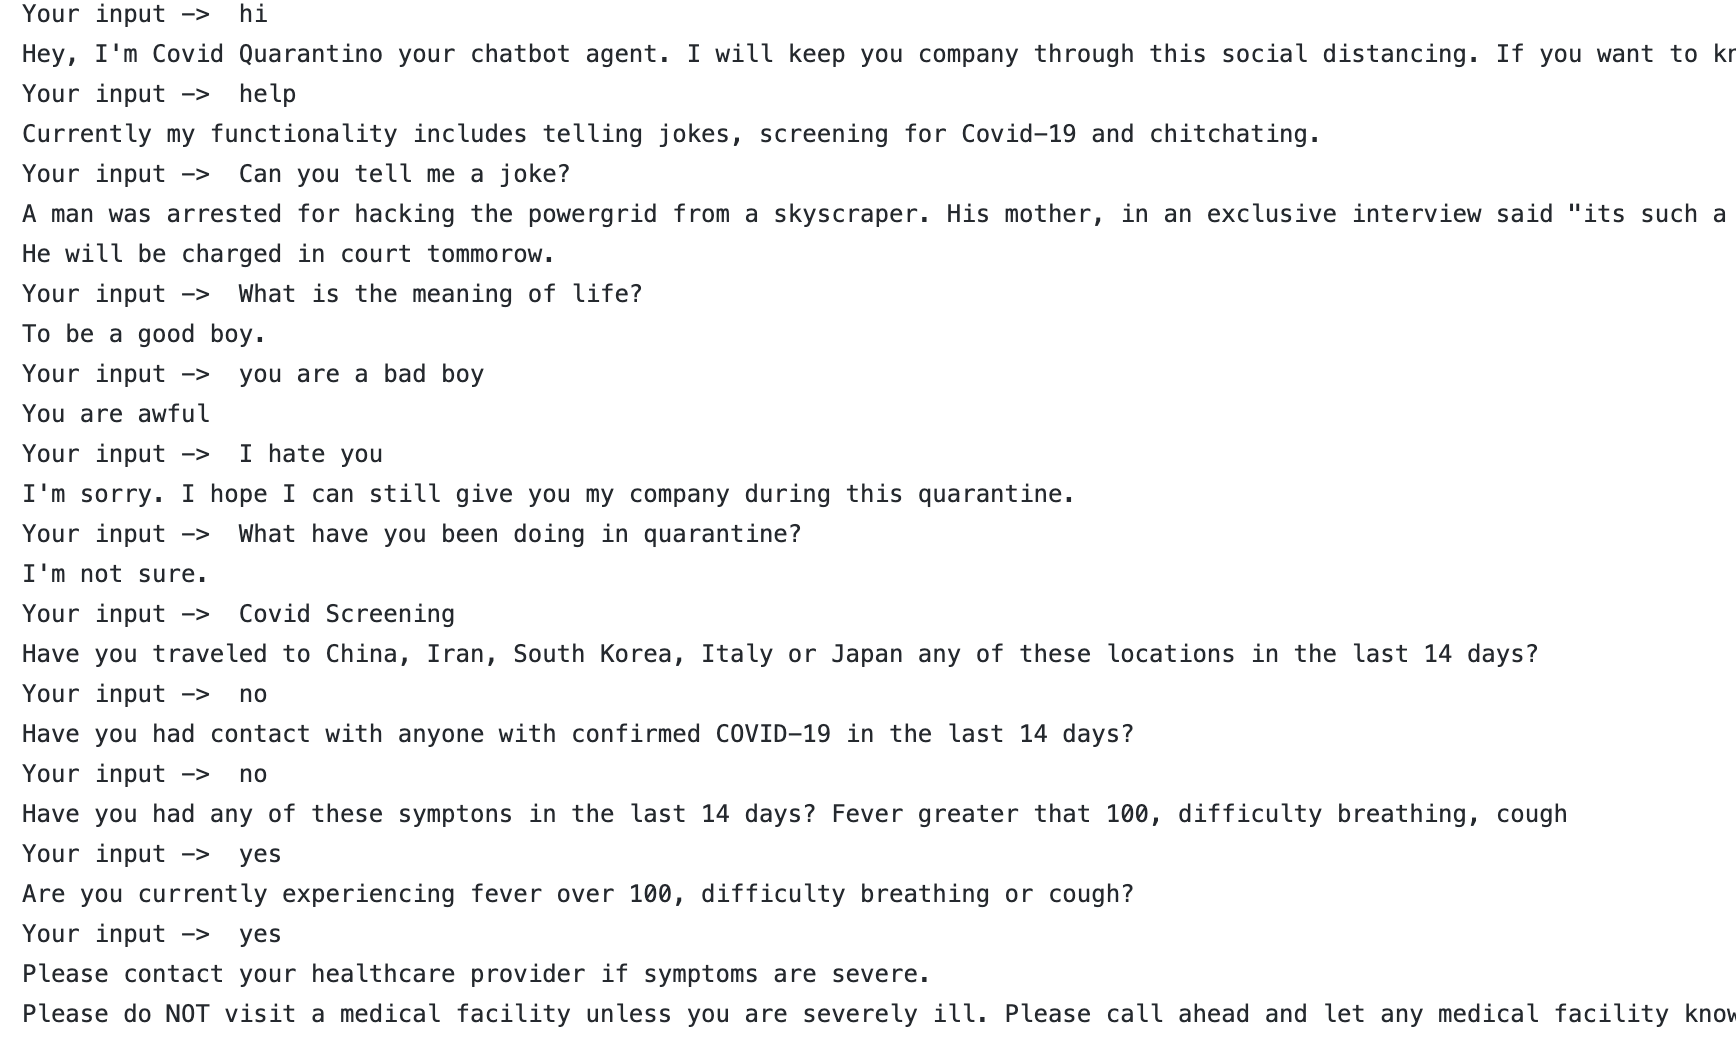
\includegraphics[scale=0.5]{conversation.png}

Notice how Covid Quarantino is able to sustain a general conversation with the user, as well as provide specific information about a topic, e.g. when prompted with \texttt{Covid Screening}.

\section{Github repo}
https://github.com/felmoreno1726/CovidQuarantinoBot

\end{document}
